\section{Современные тенденции в дизайне логотипа: культурологический аспект}

В заключение первой главы мы сделали вывод о том, что экспонента, смысловое содержание логотипа
находятся в прямой зависимости от конкурентоспособности компании-производителя  и производимых ею
товаров и услуг.  Конкурентная борьба стимулирует производителя постоянно искать и находить новые
пути эффективного сбыта продукции. Массовое производство, массовое потребление и массовая культура
естественным образом предполагают массовое производство, распространение и закрепление в массовом
сознании знаков мгновенной идентификации -- логотипов. По этой причине именно оригинальный, необычный
лого дизайн в обязательном порядке входит в бренд-пакет современных маркетинговых стратегий. По
словам британского патриарха рекламного бизнеса Д. Огилви: <<If it doesn’t sell, then
it’s not creative>>.

лого дизайн, как одна и разновидностей современного графического дизайна, есть процесс отбора и
организации графических элементов с целю достижения тройного эффекта:
\begin{enumerate*}[label=\asbuk*)]
\item <<заражать>> потребителя;
\item создавать приятные эмоции;
\item вызывать и поддерживать желание регулярно приобретать товары данного производителя.
\end{enumerate*}

Соответственно, следует различать три задачи и три функции и лого дизайна:
психологическая, эстетическая и практическая. Лого дизайнер, как показывает опыт, и как мы
проиллюстрируем в этой главе, подходит к решению этих задач эвристически и по большей части
эклектично, заимствуя идеи, приемы и композиционные решения отовсюду. Так, например, в художественном плане современный лого дизайнер нередко ассимилирует в своей практике принципы модернизма, в художественное пространство которого <<органично входят композиция, ассоциация, диссонанс, коллаж, фрагментарность>> \autocite[][322]{edoshina2002} . В содержательном же плане,
ориентированном на массовое потребление и мифопорождение, акцент делается часто на
сентиментальность, сюжетность и занимательность, на отрешенность от реального мира и
метаисторичность. \autocite{book:konradova} Они позволяют сравнительно быстро и легко завладеть эмоциональным состоянием человека на какое-то время и даже могут выполнять своеобразную психотерапевтическую функцию.

Таким образом, в данной части работы мы рассмотрим логотип с точки зрения практиков лого
дизайна. Для этого мы сначала обратимся к тенденциям в современном лого дизайне, затем перейдем к
вопросу о проблеме классификации логотипов и их типологии по идеологическим критериям счастья,
успеха и престижа.

\subsection{Культурологический анализ тенденций в современном дизайне логотипов}
Ближайшие актуальные тенденции в лого дизайне принято называть трендами. Тренд -- это один из самых распространенных инструментов организации потребительской активности в массовом обществе, с одной стороны, и обязательный предмет аналитических исследований процессов массовизации в культуре, с другой. Тренд, как правило, краткосрочен и изменчив подобно моде. Содержательно он представляет собой некоторую совокупность текущих предпочтений и приоритетов как в отдельно взятой социальной группе или среде, так и в обществе в целом. Как многое в массовой культуре, тренд может оцениваться общественностью как положительно, так и отрицательно. Конкретный <<трендовый>> (модный) товар, стиль, манера поведения, субкультура и т.п. на какое-то время уверенно завоевывает авторитет у одних категорий потребителей и вызывает стойкое неприятие у других. Тренд, запущенный в массовое производство, как показывает опыт, быстро утрачивает свое влияние и девальвируется в глазах озабоченного статусом массового потребителя.  

\begin{figure}
  \centering
  
\includegraphics[width=.3\linewidth]{images/unilever}
  \caption{Логотип «Unilever»}
  \label{fig:unilever}
\end{figure}

Тренды в дизайне логотипов, разумеется, разделяют общую участь модных веяний в массовой культуре. Так, оригинальные логотипы, становясь трендами на рынке и в профессиональной среде и, попадая затем в тираж и серийное производство, нередко могут получать негативную оценку не только от обычных потребителей, но и от взыскательных профессионалов. Например, логотип известного мирового бренда <<Unilever>> (см. рис.~\ref{fig:unilever}), который состоит из 25 иконок, образующих букву <<U>>, породил множество подражаний на рынке масскульта и лег в основу целого направления в дизайне логотипов. А поскольку значимость знака обратно пропорциональна частоте его встречаемости, логотипы, напрямую использующие этот приём -- множество элементов образует единое целое -- неизбежно становятся чем-то вторичным, а, значит, и мало интересным. Проиллюстрируем этот тезис.

\begin{figure}[h!]
  \centering
  
\includegraphics[width=.3\linewidth]{images/tutti}
  \caption{Логотип «Tutti i fiori»}
  \label{fig:tutti}
\end{figure}

Логотип цветочной студии <<Tutti i fiori>> (см. рис.~\ref{fig:tutti}) -- это попытка автора сделать эстетически красивый и гармоничный знак. Название компании переводится с итальянского как <<все цветы>>. Множественность уже подразумевается в самом названии, поэтому следование тренду здесь весьма оправданно. Однако, несмотря на то, что знак выполнен по тому же принципу, что и <<Unilever>>, он всё же имеет своё собственное лицо. Лёгкое нарушение сбалансированной формы шара за счёт вылетевшей бабочки и пары лепестков делают его более живым и динамичным. Пастельные цвета приятны для глаза, и, наконец, лигатура <<fi>> добавляет уникальности фирменному наименованию.

\begin{figure}[h!]
  \centering
  
\includegraphics[width=.3\linewidth]{images/taurica}
  \caption{Логотип <<Taurica Trails>>}
  \label{fig:taurica}
\end{figure}

Логотип компании, занимающийся экотуризмом <<Taurica Trails>> (см. рис.~\ref{fig:taurica}), отличается от <<Unilever>> главным образом тем, что название фирмы включено в общую композицию знака. Кроме того, линии-дорожки, обрамляющие слово <<trails>>, а также линии в самом знаке -- это интересная визуальная находка, благодаря которой происходит единение графики и текста. Ритмичность элементов логотипа роднит знак с орнаментом и придаёт компании этнический флёр, который также присутствует в древнем названии Крыма (Таврика). Так логотип становится эмблемой.

\begin{figure}[h!]
  \centering
  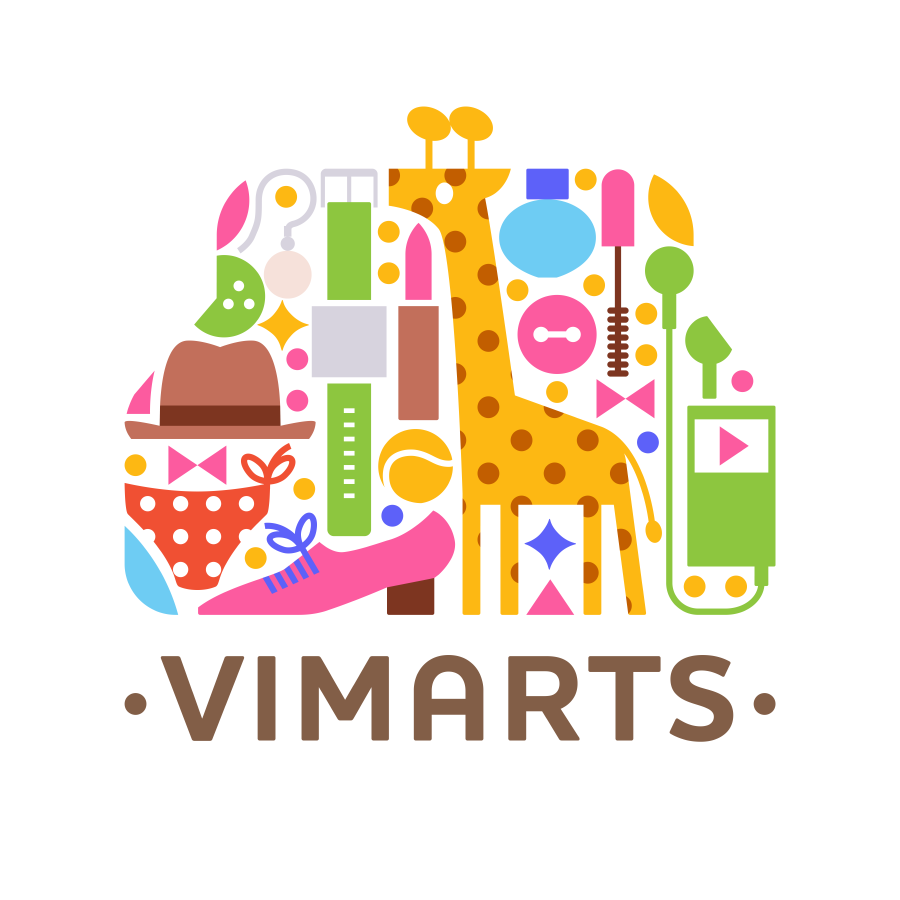
\includegraphics[width=.3\linewidth]{images/vimarts}
  \caption{Логотип <<Vimarts>>}
  \label{fig:vimarts}
\end{figure}

В случае с логотипом сайта коллективных покупок <<Vimarts>> (см. рис.~\ref{fig:vimarts}) на первый план выходит шуточная идея. Логотип наполнен пёстрыми и разнообразными вещами: губная помада, туфля, часы, тушь для ресниц, серьга, духи, теннисный мяч, плеер с наушниками, пуговица, женские трусы, мужская шляпа, шар для боулинга, игрушечный жираф. Именно жираф является здесь главным смыслообразующим элементом, рожки которого подчёркивают форму женской сумочки-кошелька. Остальные элементы служат обрамлением этой идеи. Само изображение сумочки, в которой вечный беспорядок и хаос -- это весьма типичный и узнаваемый мотив для женской целевой аудитории.

Таким образом, всякий тренд в дизайне логотипов требует от дизайнера осмысленной и оригинальной интерпретации. Оригинальность может проявляться в выборе формы, нюансе, аутентичной графике, и, конечно же, в социокультурной идее знака. Выход за рамки обыденного, изображение того, что массовая аудитория не ожидает увидеть -- сюрприз -- одно из ключевых качеств успешного логотипа. Логотип, который удивляет зрителя, застаёт его врасплох, обладает сильным эмоциональным воздействием и, в свою очередь, имеет больше шансов отпечататься в сознании потребителя.

Примечательно, что логотипы сегодня разрабатываются не только для традиционных хозяйствующих субъектов. Все чаще к самоидентификации через логотипы -- своего рода добровольному брендингу -- обращаются города, некоммерческие организации и  конкретные персоналии в социальных интернет сетях. Facebook, Twitter, Linkedin настойчиво рекомендуют пользователям использовать знаки визуальной идентификации: аватары, персональные лого, монограммы и т.д.

На сегодняшний день анализом современных тенденций в лого дизайне занимаются как простые дизайнеры-практики, так и профессиональные аналитики и критики культуры. Ниже мы предлагаем сначала срезовый анализ тенденций в
лого дизайне за периоды 2011-2012 гг. и 2012-2013 гг,  предложенных двумя профессиональными
аналитиками Биллом Гарднером и Джеймсом Боуи. Затем перейдем к более широким социокультурным
тенденциям, формирующим реалии современной массовой культуры.

Б. Гарднер занимается техническим анализом мировых тенденций в лого дизайне, в то время как  Д. Боуи
обращает большее внимание на динамику вкусовых предпочтений в американском обществе. Выбор этих двух
специалистов обусловлен их признанным авторитетом в области лого дизайна,  высокой квалификацией и
широким опытом работы в графическом дизайне.  Выбор США в качестве аналитической платформы
обусловлен  тем, что именно американский лого дизайн на сегодняшний является главным законодателем
мод, равно как и источником новых идей и влияний на практику дизайна во всем мире.

\subsubsection{Тенденции в дизайне логотипов (по Биллу Гарднеру)}

Биллом Гарднер -- директор компании <<Gardner Design>>, автор и основатель проекта
\url{LogoLounge.com}. LogoLounge.com -- это электронная библиотека логотипов, располагающая обширной и
пополняющейся базой: более 206 000 на сегодняшний момент. Логотипы для ежегодного отчёта
предоставляются известными брендинговыми агентствами и фрилансерами, любителями и профессионалами в
целях саморекламы. Тренды публикуются в течение последних 10 лет (2003-2013) и представляют собой
компилятивные иллюстративно-аналитические сборники профессионального назначения, организованные по
категориям отбора. Так, тренды 2013 года -- это результат отбора более чем 20 000 логотипов.
\autocite{link:logolounge2012}\autocite{link:logolounge2013}

Детально остановимся на тенденциях в лого дизайне на 2012-2013 гг.
(см. Приложение \ref{app:logotrends}). Предлагаемые категории: кластеры иконок-пиктограмм,
прозрачные цепочки, акварель, чипсы, анаглифы, выборочная резкость, ткань, завитушки, ростки,
кожура, резьба в сферах, мозаики, закрученные дуги, братские серии, скевоморфизм, молекулы, формула,
петля, моноширная линия.  Мы их располагаем по двум группам: переосмысление традиционных приемов
и инновации и снабжаем кратким комментарием.

\paragraph{Переосмысление традиционных приемов}
\begin{itemize}
\item \emph{Прозрачные цепочки}. Объединение множества элементов в логотипе -- давно применяемая
  практика. \textbf{Новое решение}: соединять элементы изображения в <<цепи>> по принципу
  прозрачности. Не важно, объединены ли они в круг или линию, концепт всегда один. Дополнительно
  используется эффект наложения легкого, светлого цвета приятных ощущений, через изображение
  прозрачности и взаимосвязи элементов.
\item \emph{Закрученные дуги}. Традиционные  геометрические элементы в логотипах -- простые
  прямоугольники, круги, треугольники и их комбинации. \textbf{Новое решение}: по аналогии с
  <<чипсовым>> трендом изображать  прямоугольники,  загнутые на 90 градусов и закрученные
  одновременно. Усложненные элементы-дуги объединяются и выстраиваются в замысловатые композиции,
  символизируя динамику и цикличность движения.
\item \emph{Моноширная линия}.  Для обеспечения цельности и единства системы и в качестве структурного
  элемента этот прием первоначально использовался в системах визуальных знаков и пиктограмм,
  созданных в последнее годы, предположительно под влиянием известного американского художника
  Чарли Харпера. \textbf{Новое решение}: создавать изображения  (черно-белые или цветные), где
  изображение и шрифт выполнены линией одной ширины. Возникающее герметичное изображение
  удовлетворяет композиционные потребности  формальной организации, рассчитанной на яркое
  эстетическое впечатление и запоминаемость.
\end{itemize}

Три момента обращают на себя внимание в данной группе. Во-первых, работа с абстрактными
символами. Во-вторых, усложнение композиции. В-третьих, малочисленность этих подходов. Последнее, по
всей видимости, связано с типичными недостатками пиктограмм и абстрактных символов. К таковым, в
частности, можно отнести:
\begin{enumerate*}[label=\asbuk*)]
\item малопонятность неосведомленным лицам,
\item будучи абстрактными фигурами, они требуют письменного пояснения для облегчения восприятия,
\item для их широкого использования в качестве логотипа необходимы значительные финансовые
  вложения и широкомасштабная рекламная кампания.
\end{enumerate*}

\paragraph{Инновации}
\begin{itemize}
\item \emph{Акварель}. Оформился лишь в 2012 г. в качестве альтернативы повсеместному увлечению
  технологическими решениями в композиции. \textbf{Решение}:  приблизить изображение к ощущению
  природного, человеческого восприятия либо с помощью художественной кисти из белки либо цифровым
  фильтром.
\item \emph{Чипсы}. \textbf{Решение}: использовать типическую форму закрученного картофельного
  чипса, известной в науке как гиперболический параболоид. Изображения принимают вид круга или
  эллипса, но с легким поворотом, создавая намёк на трехмерный объект. По замыслу, при восприятии
  создаётся ассоциативный ряд качеств гибкости и эластичности, впечатление, что знак сейчас
  вырвется и под действием физических законов вернется в первоначальную плоскую форму.
\item \emph{Анаглифы}. \textbf{Решение}: использовать оптическую технику смещения красного и
  синего изображений, изобретенную во Франции в 1850-е годы. Если посмотреть на такое изображение
  через грань конкретного цвета, можно увидеть либо одно, либо другое изображение. Логотип должен
  как бы говорить потребителю, что тот может сделать только один выбор, но никак не оба
  одновременно. Тем самым знак возлагает ответственность и право выбора на самого потребителя.
\item \emph{Выборочная резкость}. \textbf{Решение}: использовать современные цифровые программные
  средства для создания оригинальных изображений с драматической доминантой подобно цифровому
  фотоснимку.
\item \emph{Ткань}. \textbf{Решение}: в изображении объединять разнонаправленные векторы в единую
  плоскость, подобно тому, как нити объединены в полотно.
\item Завитушки. \textbf{Решение}: разбивать простые монотонные формы и разнообразить их цветовое
  решение, стилизуя манеру рисования линий ребенком, для создания впечатления трехмерности без
  применения градиентов.
\item \emph{Ростки}. \textbf{Решение}: визуализировать процесс органического прорастания ростка из
  семени для построения ассоциации с новым движением, зарождением, развитием, ростом и т.д.
\item \emph{Кожура}. Изначально прием двойных наклеек использовался в рекламном дизайне и позже
  был заимствован веб-дизайнерами для решения своих задач. Теперь его копируют и
  лого дизайнеры. \textbf{Решение}: создать образ, вытроенный по принципу имитации элементов
  реального мира, чтобы как бы заглянуть за кулисы, приоткрыть скрытый смысл или даже
  продемонстрировать многогранность.
\item \emph{Резьба в сферах}. \textbf{Решение}: создать изображение,  напоминающее по технике
  исполнения китайскую резьбу на шарах из слоновой кости. Сферы призваны символизировать
  глобальность мышления, а абстрактные решения внутри демонстрировать наличие многочисленных
  положительных качеств, их комплексность и сложность.
\item \emph{Мозаики}. В лого дизайне данный прием первоначально оформился в виде пиксельного
  тренда (2011 г.). \textbf{Решение}: собрать несколько геометрических фигур в картины
  повторяющихся узоров разной степени сложности. Часто элементы имеют общую цветовую гамму для
  получения эффекта наложения и прозрачности. Ожидаемое впечатление -- сила в количестве,
  многогранности, точности, кропотливости и аккуратности.
\item \emph{Братские серии}.  \textbf{Решение}: создать серию логотипов, объединенных единой
  графической формой, где каждый элемент получает индивидуальное стилистическое решение. Особую
  популярность серии приобретают в контексте разработки  бренд-программ по созданию корпоративной
  идентичности городов и территорий, о которых мы будем говорить позже.
\item \emph{Скевоморфизм}. \textbf{Решение}: имитировать в изображении дизайн схожего артефакта,
  сделанного  из другого материала. Копироваться может не только форма, вид (например, симуляция
  поверхности кожи, металла, дерева), но и функция, такая как, например, листание страниц в
  устройствах для чтения электронных книг.
\item \emph{Молекулы}. \textbf{Решение}: используя цветовую вариацию изображать геометрические
  круги, связанные линиями. Предполагаемый символизм: точность, производительность, гармоничность
  работающих вместе частей большого бизнеса, показывающих потребителю как важен процесс для
  достижения успеха.
\item \emph{Формула}. \textbf{Решение}: сделать изображение по принципу математического уравнения
  или формулы. Формула может разворачиваться вертикально или горизонтально, но всегда в
  определенной последовательности, приводящей к результату. Элементы в уравнении, на которое
  раскладывается целое, могут быть совершенно различными, но их сочетание рассказывает потребителю
  историю и требует его активного участия для того, чтобы провести их сборку и <<получить финальный
  продукт>>.
\item \emph{Петля}. \textbf{Решение}: строить изображение по форме петли, заставляющей потребителя
  совершать небольшое путешествие, прослеживая глазами плавную, текучую линию. Предполагаемый
  ассоциативный комплекс должен стимулировать представление о движении, нахождении в пути,
  достижении пункта назначения.
\end{itemize}

В данной группе сразу же бросается в глаза разнообразие оригинальных приемов и вариативность
перспектив в построении изображений с учетом его зрительного восприятия. Точно так же как и в первой
группе четко прослеживается тенденция к усложнению композиции и наращиванию символических обертонов
в плане коммуникативных ожиданий, имеющих общее, неспецифическое значение. Упор делается, во-первых,
на придание индивидуальности не только самому логотипу, но и тому, что он представляет. Во-вторых,
на искусное сочетание печати, графики и образа. В-третьих, на быстрое запоминание и уникальность.

Перейдем к обзору американских трендов.

\subsubsection{Тенденции в дизайне логотипов по Джеймсу Боуи}

Джеймс Боуи, автор популярного блога Emblemetric.com, занимается анализом трендов в лого дизайне,
используя  количественный анализ данных Офиса Патентов и Торговых Марок США. Работая с базой данных,
в которой,  начиная с 1884 г., собрано более 1 200 000 логотипов, он изучает  направления развития
лого дизайна в различных областях, включая аспекты, связанные с возникновением новых цветовых
решений композиции, рождением новых и исчезновением старых стилей, географией
покрытия. Соответственно, выделяемые Боуи тенденции, как мы увидим, носят более обобщенный
социокультурный характер по сравнению с перечнем Б. Гарднера.

\begin{enumerate}
\item Уменьшение количества  типографических логотипов в производстве товаров личной
  гигиены. Согласно статистике, процент исключительно типографических логотипов имеет тенденцию к
  уменьшению, в то время как количество логотипов,  построенных на сочетании шрифта и изображения,
  постоянно растет. Так, компания <<Проктор и Гэмбл>> в 2013 году заменила свой типографический
  логотип 2003 года (рис.~\ref{fig:emblemetrics:pg2003}) на  логотип  под девизом <<Новая фаза>>
  с изображением луны (рис.~\ref{fig:emblemetrics:pg2013}). Интересно, что в новом логотипе
  используются и некоторые другие актуальные для лого дизайна тренды,  а именно, синий цвет (он
  сравнялся с красным по частоте встречаемости в логотипах) и форма круга, популярность которой
  заметно возросла в последние годы.
\item Замена изображением отдельных букв и буквосочетаний в слове. Среди элементов, которые
  используются в этой роли, преобладают звезды, сердца, изображения земного шара, то есть элементы,
  которые не только являются популярными символами, но и могут с легкостью заместить буквы <<о>> и
  <<а>>. А такие элементы, как застежки-молнии, скрепки, наручники и пуговицы встречаются в подобных
  логотипах гораздо чаще, чем в простых графических (рис.~\ref{fig:emblemetrics:frankenmarks}).
  Любопытно, что дизайнеры таких лого зачастую мало озабочены тем, чтобы изображения, которые они
  используют вместо букв, действительно напоминали по форме эти буквы. В результате, потребитель,
  читающий такое название, вынужден самостоятельно заполнять возникающие пропуски в словах. Это не
  представляет труда в случае широко употребляемых слов. С другой стороны,  разборчивость менее
  известных слов может быть поставлена таким приемом под угрозу.
\item Отказ от абстрактных логотипов в пользу реалистических. По данным Джеймса Боуи в 2011 году
  только 36\% американских логотипов были абстрактными, остальные 61,8 \% -- реалистичными
  (рис.~\ref{fig:emblemetrics:abstract-realistic}). При этом абстрактные логотипы преобладали в
  таких сферах, как телекоммуникации, страхование, фармацевтика, химическая промышленность и
  производство металлов (рис.~\ref{fig:emblemetrics:high-abstract}). Реалистические логотипы
  использовались для продажи алкогольных и безалкогольных напитков, табачных изделий, в сельском
  хозяйстве и индустрии гостеприимства (рис.~\ref{fig:emblemetrics:high-realistic}).
\item Мотив ленты. По данным Офиса Патентов и Торговых марок США в последние годы наблюдается резкое
  увеличение количества логотипов, использующих мотив ленты в своей композиции. Петельки из ленточек
  разного цвета служат в Америке для сбора средств для всевозможных благородных целей: борьба со
  СПИДом, профилактика рака груди, поддержка американских войск за границей и многое
  другое. Преобладающими цветами таких знаков являются синий, красный, розовый, зеленый и желтый
  (рис.~\ref{fig:emblemetrics:color-use}).
\item Гендерные тенденции. По статистике три из четырёх логотипов, которые содержат какой-либо
  гендерный элемент, используют символику, ориентированную на мужчин и с включением изображений
  мужчин (рис.~\ref{fig:emblemetrics:male-female}).
\item Цвет. В цветовой палитре явными лидерами в американском обществе являются красный и синий. В
  тоже время заметен рост популярности зеленого цвета, что, по-видимому, объясняется  озабоченностью
  американского общества экологическими проблемами. Новая тенденция -- повышение интереса к
  оранжевому цвету (рис.~\ref{fig:emblemetrics:color-industry}). Анализ отраслевых цветовых
  предпочтений показывает, что красный чаще всего используется в логотипах напитков и индустрии
  гостеприимства и реже всего в страховании и медицинских услугах. Если  синий цвет предпочтителен
  для  телекоммуникаций и страхования, то в гостиничном бизнесе и туристском сервисе он используется
  не часто. Наконец, химическая промышленность чаще использует зеленый цвет, а вот страхование его
  применяет, напротив, редко (рис.~\ref{fig:emblemetrics:color}).
\item Форма. Геометрические формы, как видно и в описании Б. Гарднера, один из основных элементов
  лого дизайна сегодня. Они встречаются столь часто, что со временем их использование превратилось в
  банальность, штамп. Анализ данных Офиса Патентов и Торговых Знаков США показывает, что  количество
  логотипов с использованием основных восьми геометрических форм (круги, овалы, треугольники, ромбы,
  квадраты прямоугольники, четырехугольники и многоугольники -- пять и более  углов)  в период с
  1950 по 2010 год постоянно оставалось примерно на одном уровне -- более 50\% от всего числа
  логотипов. При этом самыми популярными формами были круги и прямоугольники
  (рис.~\ref{fig:emblemetrics:shape-industry}). Тенденция последних лет показывает большую
  популярность кругов. Они наиболее популярны в логотипах здравоохранения и телекоммуникаций и
  гораздо реже используются в страховании. Химическая промышленность чаще, чем другие отрасли,
  предпочитает треугольники, ромбы и многоугольники. Квадраты можно чаще всего увидеть в логотипах
  страховых компаний и гораздо реже в логотипах напитков. Кроме того, есть основание предполагать,
  что количество квадратов, в силу их сочетаемости  с новыми формами айдентики, такими, как фавиконы
  (значок веб сайта или веб страницы) и фотографии профилей пользователей социальных сетей, судя по
  всему, будет продолжать  перспективы  для дальнейшего роста (рис.~\ref{fig:emblemetrics:shape}).
\item Логотип веб. 2.0. Особенность этого явления  заключается в переходе веб эстетики в сферу
  традиционной двухмерной графики. Сам термин перешёл в практику дизайна из
  программирования. Говоря упрощённо, веб 2.0 -- это переход от статичного одностороннего интернета
  (веб 1.0) к интернету интерактивному, который, прежде всего, нашёл своё отражение в новых сервисах
  -- социальных сетях, блогах, торрентах, Википедии. Появление термина принято связывать со статьей
  Тима О'Рейлли <<What Is Web 2.0>> от 30 сентября 2005 г. Цифры 2.0 в названии обозначают новый
  этап в развитии интернета. Естественным образом эти процессы должны были получить новую
  визуализацию. Примерно в это же время в дизайнерском сообществе возникло повальное увлечение
  градиентами и бликами в веб и графическом дизайне. Вызвано это было новыми технологическими
  возможностями, как самих компьютерных программ, так и многократным повышением разрешающей
  способности печатных носителей. В лого дизайне этого периода и веб-дизайне стали преобладать
  округлые формы, яркие цвета, имитация глянцевого пластика современных гаджетов. С этим временем
  связана и тенденция значительного увлечения размера шрифта по значимости содержания. По сути дела,
  эта тенденция до сих пор является альтернативой классическому плоскому знаку. Сегодня мы можем
  наблюдать, как многие компании создают и обновляют свои знаки, руководствуясь принципами веб
  2.0. Так, например, этот тренд часто работает в таких сферах, где нужно показать технологичность
  или новизну товара или услуги, например, логотипы операторов сотовой связи -- Sony Ericsson,
  Megafon, Beeline, AT\&T (рис.~\ref{fig:emblemetrics:web20}).
\end{enumerate}

Таким образом, мы кратко обрисовали общие новые тенденции в движении современной дизайнерской мысли
в той ее части, где лого дизайнер принимает решение о том или ином техническом способе выполнения
задания и воплощении своего замысла. Обобщенно самые главные:
\begin{enumerate*}[label=\arabic*)]
\item Расширенная практика использования приемов синтеза, мозаичности и коллажа.
\item Постепенное вытеснение шрифтовых элементов в изображении и замена их знаком-образом.
\item Активное заимствование приемов и принципов композиции из смежных областей, особенно компьютерной графики и веб дизайна.
\end{enumerate*}

Другая тенденция, и шире -- массовая  востребованность  прикладного лого дизайна -- связана с
повсеместным распространением  маркетинговых стратегий ведения корпоративного бизнеса на организацию
жизни общественных институтов, сообществ и объединений, городов и территорий внутри страны. Здесь мы
снова оказываемся перед необходимостью объединения логотипа с его мифологизированным двойником --
брендом. Напомним, хотя логотип, как мы говорили в первой главе, филогенетически и стратегически
связан с брендом, сам он таковым не является. С другой стороны, мистическая аура бренда,
превращенного в фетиш маркетинговой риторикой, постоянно провоцирует реакцию некритичного
отождествления понятий в массовом сознании. Потому в следующем разделе мы на время согласимся с
таким словоупотреблением и будем пользоваться терминами как эквивалентами. Переходим к
территориальному брендингу как тенденции в лого (бренд) дизайне.

\subsubsection{Территориальный брендинг}

Территориальный брендинг, брендинг стран и городов, цель которого -- измерять, выстраивать и
управлять репутацией места или территории, связан в первую очередь с процессами
глобализации. Идеологи новой концепции провозглашают  новый мир  космополитичным и единообразным.
Национальные границы в таком мире постепенно утрачивают смысл, и, как следствие, встаёт вопрос о
необходимости глобальной самоидентификации --  населенного пункта, города, страны  для успешного
решения экономических, политических задач, организации культурного развития, досуга и отдыха
граждан. Показательно, что сегодня в западном мире помимо традиционного герба и флага многие
территориальные общности имеют ещё и логотип -- визуальный образ бренда. Глобальный процесс создания
новых знаковых систем идентификации происходит практически повсюду: в Америке, Европе и Азии,
России, Австралии, Африке и т.д.

Жизнь термину <<брендинг мест>> дал британец Саймон Анхольт, независимый советник по вопросам
политики из Великобритании в 1998 г. По его замыслу территориальный брэндинг в терминах
корпоративного маркетинга должен включать шесть приоритетных направлений: туризм, экспортные бренды,
политику, бизнес и инвестиции, культуру, людей. Благодаря различным каналам коммуникации бренд
должен быть понятен всем, независимо от культурных, национальных, языковых и религиозных
различий. Специалист в области территориального маркетинга и брендинга Кейт Динни формулирует это
так на примере города: <<Речь идет о стоящей перед брендами городов задаче определить их идентичность
и имидж. В чем суть города и как, с его точки зрения, ее должны воспринимать? Это нужно прояснить в
достаточной степени на начальной стадии создания бренда. Иначе мы, скорее всего, получим не внятный
бренд города, а не связанные между собой фрагментарные суббренды, каждый из которых будет нести
собственное сообщение. Но еще хуже отсутствие сознательного брендинга в принципе. В таком случае
репутация города полностью зависит от благосклонности враждебного или равнодушного
мира>>. \autocite[][127-128]{book:dinni}

Таким образом, бренд города, как некоторая  целебная общность впечатлений и представлений в головах
горожан и как его репутация, формулируется на языке торговли  как единственно возможная форма
спасения в конкурентном корпоративном мире. Репутация города оценивается согласно универсальному
бренд-индексу (City Brand Index -- CBI) по шести параметрам: внешний облик, расположение,
инфраструктура, людские ресурсы, динамика жизни, потенциал. Внешний облик, упаковка города-товара
выходит на передний план,  и вместе с ним сакрализуются визуальные образы и символика репрезентации
для создания привлекательной картинки, фасада. <<Способность графического дизайна влиять на
восприятие, эмоции, отношение людей представляет собой основной ресурс, который лица, принимающие
решения, могут использовать для того, чтобы создать крепкую, характерную для города идентичность
бренда>>. \autocite[][267]{book:dinni}

Примечательно, что традиционные геральдические знаки при таком подходе оказываются как бы
невостребованным. С одной стороны, для разработчиков бренда города эмблема (герб) является
сокровищницей информации, поскольку динамика, персоналии, элементы, цвета обычно имеют ясную
трактовку и выражают квинтэссенцию истории города, его культурным наследием. А история, в свою
очередь, является одной из главных составляющих идентичности любого места. С другой стороны, нужно
признать, что на идентичность города оказывают значительное влияние и события, произошедшие уже
после официального принятия эмблемы (герба). Строгие правила геральдики также далеко не всегда
позволяют выразить предполагаемую суть города. В результате, именно историческая направленность
эмблемы (герба) не позволяет просто переименовать ее  в логотип.

К другим ограничениям в условиях Российской Федерации также следует отнести, во-первых, правила
использования герба, которые утверждаются каждым городом самостоятельно. Чаще всего, по закону,
любое использование герба, помимо различных официальных государственных носителей, включая
праздники, необходимо согласовывать с городской думой.  Во-вторых, согласно статье 1259 <<Объекты
авторских прав>> гражданского кодекса РФ от 18.12.2006 N230-ФЗ  эмблема (герб), в отличие от
логотипа, не является объектом авторских прав: <<Не являются объектами авторских прав: [\ldots] 2)
государственные символы и знаки (флаги, гербы, ордена, денежные знаки и тому подобное), а также
символы и знаки муниципальных образований [\ldots]>> Логотип,
напротив, является объектом авторских прав. Соответственно, любая работа с логотипом строится на
договорных отношениях с его правообладателем. Наконец, эмблемы (гербы) ограничены в использовании по
их жизни на носителях. Перед лого дизайнером изначально ставится задача сделать логотип
функциональным для применения на различных носителях. Его тиражирование на различных носителях и
есть его главное функциональное преимущество.

Приведем несколько примеров успешных логотипов (брендов) городов разных стран: США, Австралии,
Европы и России.

\textbf{Логотип-слоган <<I love New York>>}

Разработанный американским дизайнером Мильтоном Глейзером в 1977 г., логотип
(рис.~\ref{fig:territorial:ny}) является одним из первых удачных и всемирно известных
территориальных брендов. Простой ребус с использование изображения сердца кажется сегодня совершенно
естественным. Округлые засечки брускового шрифта American Typewriter идеально сочетаются с формой
сердца, придавая всему образу игривый характер. В скором времени став визуальным клише, логотип
распространился по всему миру, став по степени узнаваемости и популярности приема экспортным
символом Америки, подобно бутылке Кока-Колы.

Его многочисленные копии-двойники в форме избирательных цитат встречаются повсюду. Так, например,
логотип сети книжных магазинов <<Москва>> (рис.~\ref{fig:territorial:moscow}) Ю. Шаповалова (2011)
является такой избирательной цитатой. Первая буква логотипа похожа на шрифт, используемый в
оригинале. Помимо этого, две первые буквы (M $\heartsuit$) используются в качестве отдельного
фирменного знака. Типограф Ю. Гордон пишет: <<Я склонен согласиться с автором. Действительно, если
можно считать Москву Третьим Римом, то почему бы не любить её, как второй Нью-Йорк?>>.
\autocite[][347]{book:gordon} Однако есть и отличия. Если нью-йоркский логотип выполнен одним
шрифтом, московский, наоборот, собран из разностильных букв. Такой приём демонстрирует <<широту
ассортимента книжного магазина, эклектичность московской застройки и пестроту уличной толпы>>.
\autocite[][347]{book:gordon}

В своей книге <<Christ to Coke: How Image Becomes Icon>> профессор искусствоведения Оксфордского
университета Мартин Кемп, изучая природу символа сердца, прослеживает его развитие в медицинском,
поэтическом, религиозном и коммерческом контекстах и приходит к заключению, что популярность символа
до конца не ясна. Безусловно, эта форма в силу своей простоты и соблазнительного ритма обладает
большой привлекательностью. <<Это как мелодия популярной песни>> \autocite[][110]{kemp2011christ}.

\textbf{Логотип города Мельбурн (Австралия)}

Сегодня по праву считается первым инновационным логотипом-брендом, который поднял планку и установил
новые стандарты  как в лого дизайне, так и в территориальном брендинге. Старый логотип, созданный в
конце 1980-х, был слишком повествовательным и трудным для быстрой идентификации. Он состоял из ряда
символов: М, солнце, перо, колонна, и был перегружен имплицитными значениями, что, в конечном итоге,
и послужило причиной ребрендинга в 2009 г.

Логотип был создан сиднейской студией дизайна  Landor  и сразу же имел оглушительный
успех. Повествовательность и многозначность сосредоточились в одной лишь монограмме, букве М, что
решило проблему специальной расшифровки и культурного декодирования. М -- это Мельбурн
(рис.~\ref{fig:territorial:melbourne}). Запомнить очень легко. Помимо этого, авторы разработали
красочные градиентные гаммы и правила использования логотипа в различных средах. По их замыслу,
такой подход к дизайну делает бренд узнаваемым, а вариативность графического языка соответствует
духу самого города: творческому, культурному, жизнеутверждающему.

Представление логотипа как меняющегося, динамичного знака, а также широкое использование современных
графических и стилистических приемов, сделало Мельбурн временным законодателем мод в сфере
территориального брендинга.

\textbf{Бренд-слоган Амстердама I Am -- <<Я есть>>}

Логотип (рис.~\ref{fig:territorial:amsterdam}) обыгрывает в своём названии английскую грамматическую
конструкцию.  Амстердам -- это люди, которые в нём есть. При этом не требуется никакого знака или
сложного графического образа, чтобы передать эту простую мысль. Использование ясной типографики --
буквенный логотип города воплощённый в виде уличной скульптуры -- одновременно демократичен и
стандартизован. Логотип становится достопримечательностью города, вокруг него собираются люди,
общаются и весело проводят время.

Схожую концепцию воплотила в жизнь датская студия PeopleGroup, представившая Копенгаген городом,
открытым для новых инвестиций, бизнеса и туризма. Новый логотип представляет собой игру слов, а
также акцентирование части названия зелёной кнопкой \textbf{OPEN}
(рис.~\ref{fig:territorial:copenhagen}). Авторы предлагает каждому создать
индивидуальную версию логотипа \textbf{COPENHAGEN}, приспособив её к своим целям.

\textbf{Логотип города Перми -- <<П>>}

Пермь -- первый российский город, получивший свой логотип (2009) (рис.~\ref{fig:territorial:perm}) в
общем дизайнерском пакете мер, направленных на  визуальное преображение городского ландшафта.  Город
на два года стал экспериментальной площадкой для внедрения инновационных дизайнерских идей Студии
Артемия Лебедева и Пермского центра развития дизайна (ПЦРД). За это время были сконструированы и
реализованы объекты промышленного дизайна, навигационные и  архитектурные элементы, остановки
общественного транспорта, пермские урны и т.д. Для графического сопровождения проектов типографом
Ильёй Рудерманом был разработан  специальный шрифт <<Пермиан>> и логотип города, большая красная
буква <<П>>.  В 2009 г. Марат Гельман, директор музея пермского искусства, писал у себя в жж: <<Мне
идея захватить букву ``П'' для Перми нравится даже больше чем ``А'' у Альфабанка (\ldots) Так как в
латинице такой буквы нет, появится дополнительная игра в английских текстах. Питеру ``П'' не нужна,
у них медный всадник. Остальные Пензы \ldots не успели>> \autocite{link:gelman} А также: <<Красная
``П'' чрезвычайно выразительна как дизайнерский объект. Кроме того, она похожа на силуэт старой Перми,
низковатый и плоскокрышный, но выгодно выделяется ярким цветом на фоне неброского городского пейзажа
(\ldots) С ``П'' начинается слово ``Победа'' -- почему бы не попробовать внедрить это значение в массовое
сознание. Главное, не экономить на красной краске и не забывать всё время подновлять монументальные
П-объекты. Иначе потрёпанная ``П'' обернётся в самом лучшем случае словом
``Поражение''>>. \autocite[][361]{book:gordon}

Итог. В феврале 2013, Артемий Лебедев, вспоминая годы активной работы над пермскими проектами,
резюмирует: Пермь доказала всем, что изменения вокруг возможны, но <<половину остановок так и не
подключили к электричеству, стены никто не мыл, в городе и области сменилась власть>>. \autocite{link:lebedev}

Тем не менее, творческий, если не социальный, успех дизайнеров в Перми создал прецедент и сейчас
оформился в тенденцию в дизайне логотипов городов по всей стране.  Достаточно перечислить такие
города, получившие букву в качестве логотипа, как Ярославль (рис.~\ref{fig:territorial:yaroslavl}),
Калужская область (рис.~\ref{fig:territorial:kaluga}), Невинномысск
(рис.~\ref{fig:territorial:nevinnomisk}), альтернативный логотип Омска (рис.~\ref{fig:territorial:omsk}).

Подводя итоги нашему выборочному обзору, ещё раз отметим следующее важные тенденции и особенности в
практике лого дизайна в условиях территориального брендинга в России и за рубежом.
\begin{enumerate}
\item Брендинг территорий -- это перенос способов и приемов корпоративного брендинга в общественную
  жизнь города или территории  в целях более эффективного управления их потенциалом и репутацией.
\item Потенциал места определяется, регулируется и контролируется по совокупности признаков, среди
  которых мы выделили использование систем визуальной коммуникации для решения задач
  самоидентификации -- главным образом в области лого дизайна социокультурного назначения.
\item В лого дизайне социокультурного назначения обращают на себя внимание следующие тенденции:
  \begin{enumerate*}[label=\asbuk*)]
  \item использование культурно-исторического потенциала места,
  \item его географического потенциала,
  \item создание новых знаков (абстрактных, типографических, монограмм).
  \end{enumerate*}
\item Языковые, ментальные и культурные особенности места находят свое выражении в тщательном выборе
  цветовых решений и простоте типографических форм знака-образа места. Логотип места стремится уйти
  от излишней повествовательности в сторону простого и ясного знака, понятного массовому
  потребителю-жителю-посетителю.
\item Специфика территориального брендинга в современной России на данном этапе состоит в том, что
  хотя общественность постепенно начинает осознавать потребность в обновлении визуальной городской
  среды, на практике брендинг постоянно сталкивается с объективными трудностями. По словам
  А. Лебедева, <<\ldots дизайн (\ldots) это такой род деятельности\ldots совсем избыточный. То есть,
  когда у людей все хорошо, они после этого еще думают о дизайне и тратят на него деньги. В деревне
  не нужен дизайнер. Это профессия городская, капиталистическая и от хорошей жизни возникающая,
  когда остальные проблемы решены>>. \autocite{link:plushev}
\end{enumerate}

Теперь, в завершение параграфа мы рассмотрим еще одну социальную тенденцию в лого дизайне, носящую
характер радикального отрицания. Суть радикализма – полный отказ от использования знака логотипа,
инспирированного, помимо всего прочего, протестной общественной деятельностью канадской журналистки
Наоми Кляйн, на которую мы уже ссылались в первой главе в связи с общей постановкой проблемы
логотипа.

\subsubsection{Критика логотипа-бренда}

Итак, ниже мы рассмотрим вопрос о негативном восприятии логотипа-бренда сначала антиглобалистким
движением, которое представляет собой не что иное, как классический пример стихийного массового
образования, описанного нами в самом начале исследования.

В декабре 1999 г. в издательстве <<Knopf Canada>> вышла сенсационная на тот момент книга канадской
журналистки и общественной активистки Наоми Кляйн под названием <<No Logo: Taking Aim at the Brand
Bullies>>. Газета <<Нью-Йорк Таймз>> сразу же назвала труд Кляйн <<евангелием антикорпоративного
движения>> и новым <<Капиталом>>. Книга написана в свободной манере и представляет собой синтез
экономических и культурологических наблюдений и размышлений, политический манифест и журналистское
расследование, бескомпромиссно критикующее глобализацию и современный экономический порядок мире,
опутанном сетями глобальных брендов.

Во вступлении Кляйн, в частности, пишет: <<Название этой книги, NO LOGO, не задумывалось как
воспринимаемый буквально лозунг <<Нет логотипам!>> или <<Долой логотипы!>> или как брэнд
постбрэндовой эпохи. (\ldots) Эта книга строится на простой гипотезе: по мере того как все больше и
больше людей будет открывать секреты товаров, выпускаемых под известными марками в глобальной
паутине брэндов, их возмущение будет подливать масла в огонь следующего крупного политического
течения, могучей волны оппозиции>>. \autocite[][16-17]{klein2003}

Собранный в книге материал по истории возникновения и становления наиболее крупных современных
брендов включает такие компании как Nike, Reebok, Microsoft, McDonald’s, Gap, Polo, Tommy Hilfiger и
др. На их примере Кляйн показывает переход от производства продукции к производству бренда как
самоцели. Бренд уже не привязан к какому-то конкретному товару, но организует новую сложную систему
отношений -- спонсорство, организацию благотворительных акций, меценатство и т. п. Если раньше
торговая марка имела различительную функцию на рынке товаров одного типа и связывалась, в первую
очередь, с категорией качества (что можно было видеть и в рекламе, и в способах представления
продукции потребителю), то бренд работает уже с производством иных образов жизни, стилей
существования, идентичностей, задавая совершенно иной набор социальных ценностей.

Книга разделена на четыре части, каждая из которых показывает, каким образом бренды входят в нашу
повседневную жизнь. С самого начала Кляйн последовательно показывает детальную картину захвата
брендами пространства городов и университетов. Оккупируя все новые и новые сферы влияния, бренды
формируют молодежную культуру, утверждают четкую структуру статусов через логотипы на одежде и марки
кроссовок, когда подросток включается в своего рода <<маркетинг крутизны>> и оказывается <<живым
брендом>>. Школы, университеты, улицы, публичные места кишат брендами, предлагающими множество
образов жизни, имиджей, возможностей соотнести себя с определенным социальным статусом.

Далее, Кляйн задается вопросом о месте свободы выбора внутри такого многообразия и приходит выводу,
что никакого выбора нет. (Schwartz choice anxiety!) Создавая, как нам кажется, наш индивидуальный,
неповторимый стиль, мы неизменно оказываемся вовлеченными в такую систему уже заданных возможностей
построения имиджей, становясь <<забрендованными>> маргиналами или менеджерами среднего звена. Кляйн
фактически создает нечто вроде мифологии о злых богах-брендах, борьба с которыми -- наша
первостепенная задача.

Симптоматично, что ее критика брендов основана главным образом на разоблачительном пафосе
«зомбирования» сознания в духе классической теории заговора.\autocite{entin2000} Более изощренную и
по-постмодернистски малопонятную интерпретацию влияния брендов на сознание мы находим у
академических критиков современного общества, для которых бренды уже, по-видимому, не являются
просто элементами нашего сознания.  Они фактически инкорпорированы в наши тела и служат
своеобразными инструментами контроля, о чем в свое время писали М. Фуко, Ж. Делёз и др. Контроль
осуществляется через включение человека в коммуникативные процессы, в общие информационные
зоны. Другими словами, бренд представляет собою медийный конструкт, уже апеллирующий к неким общим и
приобщающим ценностям, заключенным в истории, традиции, в общих представлениях. Пожалуй, именно в
этом общем, узнаваемом и заключается вся его притягательность. Он не работает с индивидуальным,
сфера его востребованности — это общее. Парадоксально, но помимо несвободы, против которой так резко
выступает Наоми Кляйн, бренд дает людям некоторую иллюзию общности. Следовательно, помимо
манипуляции сознанием, есть смысл говорить о коммуникативной составляющей бренда.

Действительно, выбор в условиях современного производства невозможен, но, предаваясь иллюзии выбора
и покупая одежду одной марки, а не другой, мы, как потребители, включаемся в игру иллюзий. В
частности, иллюзии стиля. С момента, когда французский естествоиспытатель Жорж Луи Леклерк Бюффон 25
августа 1763 г. при избрании его в члены Французской академии, провозгласил, что <<стиль -- это
человек>>, он являлся признаком индивидуального, тем, что определяет персональность,
личностность. Однако в современном же мире количественного прирастания бытия говорить о стиле все
сложнее, так как он уже не несет в себе традиционной социальной дифференциации, да и такие ценности
<<высокой культуры>>, как авторство, индивидуальность, личность все меньше связываются со
стилем. Стиль сегодня -- это эффект выражения, и там, где стиль, уже нет индивидуального, а есть
выражение некоей всеобщности. В этом смысле, бренд является последним эффектом стиля, создающим
<<общее место>>, в котором соединяется прежнее уютное кафе и современная огромная корпорация. Через
бренды поддерживается эстетика стиля, реализуется иллюзия различия и индивидуальности. Бюффоновское
высказывание превращается в свою противоположность: там, где стиль, там нет человека, нет
личности. Стиль бесчеловечен.

Проблема заключается в том, что традиционная критика бренда, как в случае с Наоми Кляйн, идет с
позиции обнуленного означающего, из точки его гипотетического отсутствия, что в современном мире
практически непредставимо. И критика, призывающая к борьбе против засилья брендов, во многом сама же
их и создает. Так, бренд не может быть причиной угнетения перуанских женщин, и критика,
представленная в книге Наоми Кляйн, похоже, исходит из слишком прямой связи бытования бренда в
современном обществе с условиями производства. Все дело в том, что бренд не является только
экономической категорией, он выходит за рамки идеологии потребления, выступая скорее регулятивным
социальным элементом. Критиковать бренды, наверное, это почти то же самое, что критиковать
паспортную систему. Универсализм брендов предполагает ситуацию скрытой деполитизации мира, когда
сами паспорта, удостоверения личности, выглядят уже архаично.

Примерно в декабре 1965 г. англо-американский поэт У. Х. Оден написал полусатирическое
стихотворение <<Песнь Дьявола>> (Song of the Devil), в котором главный персонаж Дьявол ставит
холодно-циничный, но точный диагноз личности потребителя в обществе потребления. Процитируем только
один небольшой фрагмент:
\begin{verse}
Поскольку люди подобны товарам, причем тут вопросы морали \\
Когда ты и есть самый Главный Бренд? \\
И пусть все заткнутся, ты все равно лучше их всех, \\
Дай им по голове, если посмеют приставать с вопросами -- \\
Мол, что Вы намереваетесь делать, \\
Или -- каковы у этого могут быть последствия: \\
Они тебе не ровня.
\end{verse}

В парафразе: поскольку люди подобны товарам, и ты, как личность, не больше ни меньше Ведущий Бренд,
нравственные ограничители неуместны, мнения других неважны. Ничего не объясняй и ни перед кем не
оправдывайся. Различие между тобой и остальными в масштабности личности. Или лучше: в масштабности
<<лича>>, редуцированной эрзац-личности, выхолощенной конструкции, лишенной живого содержания и
творческой силы. Личность, которой современная мода предлагает быть творцом собственных ценностей,
внутренне пуста, то есть вообще личностью не является. Оденовский герой называет лич-потребителя --
<<only a cypher>>, одна лишь фикция, пустое место. И если он меняется, то меняет он не себя, а образцы
для подражания. Так выглядит сформулированный современной культурой персонаж -- <<лич>>, абстрактное
существительное со значением отвлеченного качества, но уже без суффиксов -н-ость-. Вымышленный.
Похожий. Встречается только среди людей. Но культуру, думается, все-таки
нельзя отождествлять с полнотой бытия, поскольку, подменяя жизнь ее культурным отражением, мы
подвергаем себя опасности чего-то не заметить в жизни, причем подчас самого интересного и самого
важного.

До этого мы говорили о двух важных тенденциях интерпретации логотипа с точки зрения социокультурной
динамики:
\begin{enumerate*}[label=\arabic*)]
\item семиотическом расширении знака: от логотипа вещи к логотипу территории и
\item замещении личности логотипом-брендом. Теперь сделаем небольшое дополнение к и проиллюстрируем
  принцип частичного отказа от логотипа на примере анти-брендинговой стратегии японской компании
  Muji и недавней акции лондонского универмага Селфриджес.
\end{enumerate*}

Как мы уже отмечали в главе \ref{chapter1} нашего исследования, массовая культура и рынок характеризуется
избыточным потреблением товаров и услуг. Но, по всей видимости, эйфория потребления, равно как и
любое эмоциональное переживание, не длится долго. Потребитель устает от монотонности мелькающих
логотипов и брендов, от быстро меняющихся и недолговечных вещей, и наконец, от разоблачений и
утверждений, что его сознанием постоянно манипулируют. Всё это вызывает в нас чувство раздражения,
недовольства и, главное, ностальгии по старым добрым временам, когда вещи были простыми и честными,
надёжными, сделанными из натуральных материалов, без крупного логотипа. Современный маркетинг готов
помочь и в этом. В конце концов, во всех поколениях присутствует тип потребителя, избегающего всего
популярного и массового. Но это лишь говорит о том, что они принадлежат иной массовой
общности. \autocite{lindstrom2011brandwashed}  Для маркетинга
нонконформизм есть только разновидность конформизма. Проиллюстрируем двумя примерами.

Первый пример связан с отказом от эксплицитного использования логотипа по причине популярности
продукта. Знаменитый лондонский универмаг Селфриджес в начале 2013 г. проводил акцию под названием
<<No Noise>>, в рамках которой были удалены логотипы с узнаваемых жёлтых пакетов универмага, а также
был предусмотрен выпуск ограниченного количества известных продуктов без логотипов: кетчупа и фасоли
Heinz, увлажняющего крема Clinique, джинсов Levy's модели 501 и ряд других марок.

Второй пример -- японская компания <<Muji>>, специализирующаяся на изготовлении товаров для дома,
имеющая репутацию таинственного бренда, или антибренда. Muji -- сокращение от Mujirushi
Ryohin, что с японского означает <<качественные товары без этикеток>>. Примечательно, что
компания возникла в 1980 г., за 20 лет до того, как Наоми Кляйн опубликовала свой знаменитый
манифест антикорпоративного движения <<No Logo>>. Руководство компании изначально разработало
стратегию, целью которой было создание <<честного дизайна>> для пресытившегося, апатичного японского
потребителя. При этом при разработке дизайна для своей продукции функциональность вещи была призвана
заместить её образ. Вещь предоставляется покупателю такой, какая она есть, без логотипа. Товар в
магазинах разложен по пластиковым контейнерам и плетёным корзинам. На самом товаре -- одна лишь
бирка.

Не смотря на то, что имена дизайнеров, работающих на компанию, держаться в строгом секрете, некоторой информации всё же удаётся распространиться. Так, например, культовый CD-плеер, разработанный японским дизайнером-минималистом Наото Фукасава для Muji является признанной «иконой» в мире предметного дизайна. Безусловно, по формальным признакам шрифт и цвет, который использует компания для своей идентификации, и даже тот минимум упаковки является скорее  по-новому упакованной бренд-стратегией.  Логотип как эксплицитно выраженный материальный знак больше не нужен, поскольку он  оставляет свой отпечаток-бренд в сознании потребителя по иному принципу. Так, в структурной лингвистике есть понятие нулевого знака, значимого отсутствия, подобно нулю в математике, мере пустого множества. Остановимся на этом вопросе подробнее. 

Утилитарно нуль в математике максимально функционален при формировании позитивных множеств, когда он сочетается с другими положительными целыми числами. В структурной лингвистике, по Р. О. Якобсону, нуль (нулевая форма) значим по признаку отсутствия материального способа выражения.  По этому признаку он образует оппозицию с другим знаком или знаками, имеющими материальную форму. Например, «нулевой артикль» в английском языке находится в оппозиции к неопределенному и определенному артиклям (“a/n”, “the”).  А.И. Смирницкий,  автор «Морфологии английского языка» (1959) и один из первых отечественных пропагандистов нулевых форм, предлагает называть нулевым артиклем «значащее отсутствие артикля, т.е. такое его отсутствие, которое соотносится и сопоставляется с наличием определенного и неопределенного артикля».\autocite[][382]{smirnizki1959} Такое отсутствие, по его мнению, несет специфическую семантическую нагрузку. А именно: существительное, определяемое нулевым артиклем, «выступает в самом общем, широком значении и обозначаемый им предмет рассматривается лишь с точки зрения его сущности».\autocite[][383]{smirnizki1959} Но изучение сущностей денотатов не входит непосредственно в предмет изучения лингвистики, что, по всей видимости, объясняет преимущественно классификационный статус нулевого артикля в науке о языке. \autocite{berezowski2009}Вопрос сущностей –- вопрос культурно-философский. 

Понятие нуля исторически впервые возникает и получает свое развитие в древней Индии (по другим версиям, в древнем Китае). В I в. н.э. в индийской математике вводится специальный знак для нуля, и он становится полноценным числом.\autocite[][351]{stepanov2004}  В контексте индийской и шире -- азиатской культуры, полагает А. И. Степанов, понятие нуля органично. Как в индуизме, так и в буддизме, проблема значимого отсутствия является проблемой онтологической и гносеологической, наряду с пустотой и нирваной, освобождением от иллюзорности материального мира. Простое отсутствие, т.е. нуль, переходя во внутренний план рефлексии, становится методом мышления, т.е. «пустотным мышлением».\autocite[][352]{stepanov2004} Возьмем только один его аспект -- молчание, «вслушивание в тишину Истины.», попытка, по Августину Аврелию, «понять вечное Слово, пребывающее в молчании.» \autocite[][ХI, 6, 8]{avgustin1992} Молчание как вид духовной практики есть одно из важнейших духовных упражнений, известное с незапамятных времен в христианстве и получившее широкое распространение в странах Востока, исповедующих буддизм. В таком молчании рождается внутреннее слово, в котором весь мир постигается  целиком и сразу.\autocite[][112-125.]{nestik1998} Такое нетривиальное молчание есть нечто иное, как значимое отсутствие слов, или «нуль» слов. Он логически предшествует речи и ее завершает. Онтологически безмолвие, подчеркивает А. И. Степанов, является спутником величественного. \autocite[][358]{stepanov2004} \footnote{Вне религиозного контекста  в качестве генетического, хотя и значительно ослабленного,  аналога можно было бы назвать, например,  «экспрессию молчания» в публичной риторике,  или «многозначительное молчание» в нашей повседневной жизни – паузы между словами или высказываниями, пробелы в письменном тексте и т.д.} Или, в популярной цитате С. Беккета: «Nothing is more real than nothing.» \autocite[][63]{esslin2004} Возвращаемся к нашему примеру с устранением логотипа на товаре японской компании.

В свете сказанного выше должно быть понятно, что идея ликвидации логотипа совсем не случайно возникла именно в Японии. Это не просто экстравагантный ход японских маркетологов и дизайнеров, а пример адаптации западной технологии к национальной культурной традиции, придание ей самобытной формы, наполнение ее внутренними смыслами. Это пример “пустотного мышления”. Вместо тотальной саморекламы через самоидентификацию посредством логотипа -- «нуль» знаков, отсутствующая форма, значащее молчание.  Отсутствие логотипа значимо именно потому, что это отсутствие значимо онтологически. Нулевой логотип, как и нулевой знак, отсылает к сущности вещи. Тем самым он  популяризует  разумный материализм и разумное потребление.  Бренд утверждается, но он утверждается апофатически, через отрицание. Отрицается фантазийная, виртуально-магическая модель рекламной саморепрезентации, практикуемая в западном мире. \autocite[][410-423]{williams1999} 

Тем временем имена популярных логотипов-брендов откладываются не только в ассоциативной потребительской памяти, но, что важнее -- в языке.  Например,  «твитнуть» от имени социальной сети «Twitter», «отксерить» -- от названия компании «Xerox». Румынская студия Next Advertising в 2011 г. получило первое место в номинации «Телевизионная и кинореклама» на Московском международном фестивале рекламы «RedApple». Один из призовых видеороликов называется «Ревность». Он представляет собой драматургическое повествование в псевдоабсурдном ключе. Иными словами, является таким типом повествования, которое вначале может быть ошибочно принято за абсурдное, но получает рациональное истолкование в конце.\autocite{ivleva_thesis}
Мизансцена: Муж поздно возвращается домой, жена встречает его в дверях. Процитируем их дальнейший разговор:

— Nokia, Vodafone?...

— Microsoft, HP, Xerox, Post-it...

— Tuborg? Stella Artois? Bergenbier? Avon! Nescafe, Novotel, Durex?

— Microsoft, HP, Xerox...

— Domestos, Ariel, Whirlpool... Avon, Novotel, Nescafe, Durex? Novotel? Toyota, Novotel!

Разговор состоит из пяти реплик-высказываний. Три из которых принадлежат жене и две - мужу. Реплики жены заметно эмоциональнее (семь знаков вопроса, два знака восклицания) и продолжительнее (7 лексических единиц в третьей строке и 10 в пятой). Каждая единица представляет собой имя торговой марки или бренда, которые и формируют, собственно, абсурдный фон разговора. Имена брендов (всего 17) подаются в виде неких семантических блоков. Рассмотрим построчно.
Первый: имена современных европейских компаний-производителей сотовых телефонов и сотовой связи.
Второй: имена американских компаний-производителей программного обеспечения, офисной оргтехники и канцелярских товаров).
Третий: имена европейских пивоваренных компаний, американской косметики, шведского производителя кофе, бренда французской гостиничной сети и британского изготовителя барьерных контрацептивов)
Четвертый: неполное воспроизведение второго.
Пятый: имена англо-датской, американской, итальянской компаний-производителей бытовой химии и техники, американской косметики, бренда французской гостиничной сети, шведского производителя кофе, британского изготовителя барьерных контрацептивов, бренда французской гостиничной сети, японской автомобилестроительной корпорации и снова бренда французской гостиничной сети.
Визуальный ряд легко позволяет следить за развитием общей сюжетной линии в сцене, в то время как конкретное содержание реплик персонажей, его собственное речевое выражение – как это свойственно драматической технике абсурда – зрителю предлагается создать самостоятельно по ассоциативному принципу. \autocite[][189-209]{stern1990} \autocite[][72-81]{stern1992} \autocite[][35-49]{arias2000} Или же, в семиотической формулировке, сделать перевод с одного языка на другой. Например такой вариант:

-- Я тебе звонила, почему не отвечал?

-- Много работы, пришлось задержаться.

-- Пил пиво с друзьями? Ах, нет, ты был с женщиной! Сначала кофе пили, потом в отель пошли?

-- Да на работе я был…

-- Я тут весь день мою, стираю… А ты с любовницей в отелях развлекаешься? Вот и катись к ней теперь!

Ролик завершается ироничным слоганом: Реклама - часть нашей жизни. Ирония состоит в том, что реклама давно уже не является \emph{частью} жизни, а формирует ее. С другой стороны, реклама – это культурный код, знание которого позволяет \emph{читать} содержание нашего повседневного быта, вкусов и предпочтений, ценностей. Код торговых марок (брендов) – код универсальный уже по тому, что он свойственен исключительно массовому обществу, в котором люди подобно героям пьесы театра абсурда «становятся аморфными, могущими видоизменяться как угодно и сколько угодно раз».\autocite[][75]{edoshina2002} Код рекламы – это также и код массовой культуры. <<Доместос>> всегда для всех и везде будет популярным универсальным моющим средством. Логотип в свою очередь выполняет функцию мнемонического инсталлятора такого кода. Дело в том, что логотип, помимо всего прочего, семиотически представляет собой \emph{перформативный} знак, непосредственно соотносящийся с актуальной реальностью. В то же время логотип, сопровождающий успешный и популярный бренд получает потенции знака информативного, т.е. отсылающего к определенному значению или совокупности значений, образующих, по словам Б.А. Успенского, виртуальную реальность.\autocite[][9]{uspenski2007} Такая реальность составляет самостоятельное целое и функционирует независимо от конкретных денотатов. Она так же лежит в основе языковой картины мира и массового сознания как такового.
Обобщим.

\begin{enumerate}
\item Мы представили тенденции в современном лого дизайне по двум направлениям: узкопрофессиональные
  технические предпочтения и инновации, с одной стороны, и социокультурные изменения,
  переопределяющие традиционно корпоративное, коммерческое  назначение логотипа -- с другой.
\item Тенденции в новых технических решениях дизайна логотипов, мы показали, свидетельствуют о двух
  ясно выраженных предпочтениях:
  \begin{enumerate*}[label=\asbuk*)]
  \item заменять отдельные шрифтовые элементы в изображении малым
    знаком-образом,
  \item интегрировать способы и приемы виртуального дизайна в практику изготовления
    логотипов.
  \end{enumerate*}
\item Новое направление в практике лого дизайна -- разработка логотипов корпоративной семиотизации
  объектов  социальной среды в рамках программы глобального брендирования территорий в целях
  повышения внешней привлекательности конкретного территориального субъекта для индустрии туризма,
  привлечения инвестиций и модернизации инфраструктуры города или территории.
\item В отличие от зарубежного опыта брендирования, деятельность графического дизайнера в России
  сопряжена с  определенными объективными трудностями. К таковым, в частности, относятся:
  относительно низкий уровень жизни населения в массе, слабое понимание преимуществ новой стратегии
  на местах, отсутствие стабильной финансовой и политической поддержки осуществленных дизайнерских
  проектов.
\item Корпоративное видение жизни общества и действия транснациональных корпораций по
  распространению своего влияния на все уровни жизнедеятельности, как массовых общностей, так и
  каждой отдельного индивида в обществе, встречают решительной протест со стороны активистов
  движения антиглобалистов, и подвергается резкой критике со стороны влиятельных интеллектуалов
  разных стран.
\item Корпорации изобретательно используют протестные, нонконформистские настроения в обществе и
  ассимилируют их пафос в новых маркетинговых стратегиях, диверсифицирующих, как направление
  деятельности компании, равно как и предложение своего товара с учетом происходящих изменений в
  умонастроениях потребителей.
\item В качестве примера гибкости современных маркетинговых стратегий мы описали тенденцию к
  избирательному устранению знака логотипа с внешней поверхности товаров и упаковок. Тем самым
  демонстрируя потребителям:
  \begin{enumerate*}[label=\asbuk*)]
  \item свою заинтересованность в их длительной лояльности и
  \item свою осведомленность о наличных эмоциональных состояниях, предпочтениях и переживаниях в их
    психической жизни.
  \end{enumerate*}
\end{enumerate}
